\section{Algoritmo de posicionamiento de pacientes virtuales} 
\label{posing:result}
%%%%%%%%%%%%%%%%%%%%%%%%%%%%%%%%%%%%%%%%%%%%%%%%%%%%%%%%%
%\todo{No me gustan los apartados. Separa entre rendimiento y calidad}
%\todo{Pasar todos los resultados al capítulo de resultados}

%\todo{pasiva}

%En esta sección se va a proceder a mostrar los resultados obtenidos por el algoritmo propuesto utilizando distintos pacientes virtuales.
Con el objetivo de evaluar este algoritmo, se han elegido distintos modelos anatómicos.
Entre estos modelos, se incluyen modelos comerciales, otros procedentes de imágenes de pacientes reales 
%o ejemplos básicos. 
y formas geométricas básicas, que representan modelos de diferentes procedencias. Esto permitirá probar la flexibilidad del algoritmo utilizando distintos tipo de pacientes virtuales.
%Estos modelos procede representan una gran parte de la variabilidad a la que se pueda enfrentar el método propuesto. 
%A continuación se enumeran los modelos utilizados:
En la tabla ~\ref{tab:complex} se resume el tamaño de los modelos mostrados en la figura \ref{fig:models}, y la complejidad de las mallas volumétricas generadas para cada uno. Es necesario destacar las dimensiones de los modelos anatómicos y las representaciones volumétricas en comparación con los tamaños habituales 
%vistos en la sección de estado del arte 
utilizados por las técnicas descritas en la sección \ref{art:animation}. 
En ocasiones, estos modelos tienen una complejidad de un orden de magnitud superior a las utilizadas en la bibliografía citada.

\begin{table*}[ht]


\centering

\caption{Complejidad de los modelos utilizados.}
\label{tab:complex}
\begin{tabular}{|x{35mm}|x{20mm}|x{24mm}|x{20mm}|x{24mm}|}
\cline{2-5}
\multicolumn{1}{c}{ }
&
\multicolumn{2}{|c}{Malla superficial }
&\multicolumn{2}{|c|}{Malla volumétrica }
 \\
 \hline
\textbf{Modelo } 
& \textbf{Vértices }
& \textbf{Triángulos}
& \textbf{Nodos}
& \textbf{Tetraedros} \\ 

\hline
\emph{ZygoteBody}$^{TM}$ Masculino \cite{kelc2012zygote}            &1 317 862      &2 601 469   &553 412 &2 576 779\\
\hline
\emph{ZygoteBody}$^{TM}$ Femenino \cite{kelc2012zygote}         &1 468 989     &2 896 011   &492 646 &2 314 456\\ 
\hline
\emph{Anatomium} Masculino \cite{Anatomium}     &790 461     &1 570 778    &767 325 &3 411 170\\ 
\hline
\emph{Segmented Inner Organs}\cite{VoxelMan} &591 265     &1 184 325    &242 033  &1 182 485\\ 
\hline
Datos de pacientes reales     &31 987       &63 926   &82 277  &346 853\\ 
\hline
Modelo de barra con cuatro huesos  &2 152     &4 268    &8 539 &39 419\\ 
\hline



\end{tabular}

\end{table*}


% \begin{itemize}
%     \item \emph{ZygoteBody}$^{TM}$ Masculino \cite{kelc2012zygote}
%     \begin{itemize}
%         \item Vértices: 1317862
%         \item Triángulos: 2601469
%         \item Nodos: 553412
%         \item Tetraedros: 2576779
%     \end{itemize}
%     \item \emph{ZygoteBody}$^{TM}$ Femenino \cite{kelc2012zygote} 
%     \begin{itemize}
%         \item Vértices: 1468989
%         \item Triángulos: 2896011
%         \item Nodos: 492646
%         \item Tetraedros: 2314456
%     \end{itemize}
%     \item \emph{Anatomium} Masculino \cite{Anatomium}
%     \begin{itemize}
%         \item Vértices: 790461
%         \item Triángulos: 1570778
%         \item Nodos: 767325
%         \item Tetraedros: 3411170
%     \end{itemize}
%     \item \emph{Segmented Inner Organs}\cite{VoxelMan}
%     \begin{itemize}
%         \item Vértices: 591265
%         \item Triángulos: 1184325
%         \item Nodos: 242033
%         \item Tetraedros: 1182485
%     \end{itemize}
%     \item Datos de pacientes reales
%     \begin{itemize}
%         \item Vértices: 31987
%         \item Triángulos: 63926
%         \item Nodos: 82277
%         \item Tetraedros: 346853
%     \end{itemize}
%     \item Modelo de barra con cuatro huesos
%     \begin{itemize}
%         \item Vértices:  2152
%         \item Triángulos: 4268
%         \item Nodos: 8539
%         \item Tetraedros: 39419
%     \end{itemize}
% \end{itemize}

\begin{figure*}[ht]%[b]%[b!ht]
  \centering
  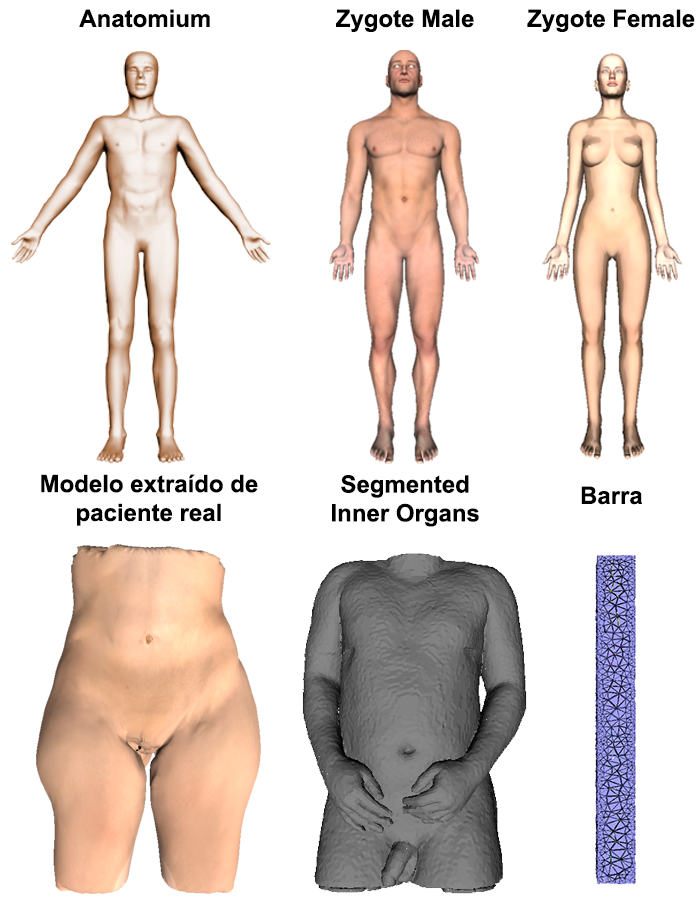
\includegraphics[width=0.90\textwidth]{IMG/modelos}
    \caption{Ejemplo de los modelos utilizados en los test.}
    \label{fig:models}
\end{figure*}

%ZM es Zygote Masculino, ZF es Zygote Femenino, A es Anatomium

Con el objetivo de no necesitar un usuario con habilidades artísticas o conocimientos avanzados de anatomía, se han utilizado animaciones procedentes de la base de datos de \emph{\ac{MoCap}} de la \emph{Carnegie Mellon University}~\cite{CMUMCD}. El computador utilizado para realizar todos los test de la presente tesis se compone de un procesador \emph{Intel\textregistered i7-4820K @ 3.7GHz}, tarjeta gráfica \emph{GeForce GTX 770} y 16GB de memoria \acs{RAM}.
\clearpage

\subsection{Análisis previo}
\label{sec:ana_prev}

%%%%%%%%%%%%%%%

En este apartado, se analizarán las principales cualidades y limitaciones del algoritmo propuesto. Inicialmente, se mostrarán los resultados de las modificaciones realizadas para mejorar la robustez del algoritmo debido a los problemas encontrados en los modelos anatómicos utilizados. Después, se realizará una comparación entre las distintas técnicas de \emph{skinning} descritas en el capítulo \ref{cap:posing}, finalizando con ejemplos de deformaciones obtenidas por el algoritmo.


Aunque el algoritmo se ha diseñado con el objetivo de ser lo más robusto posible, hay que destacar que los modelos con los que se ha trabajado no están exentos de problemas. 
%Por una parte, en 
\begin{figure}[ht]
   \centering
    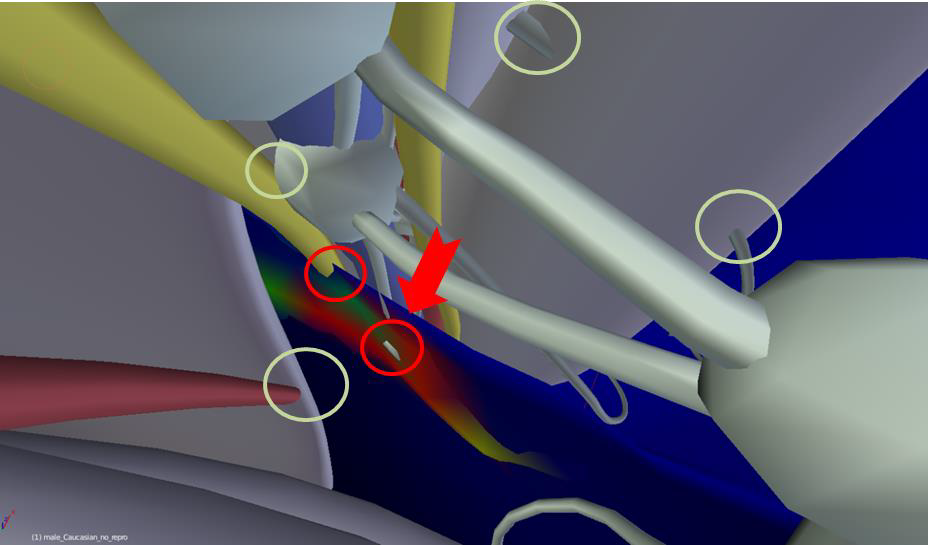
\includegraphics[width=0.85\textwidth]{IMG/zygoteproblems.png}
    \caption{Axila del modelo \emph{ZygoteBody}$^{TM}$ Masculino. Con círculos amarillos se observan colisiones entre diferentes tejidos. Los círculos rojos representan colisiones con el tejido de la piel.}
   \label{fig:zygoteproblems}
\end{figure}
Por ejemplo, ambos modelos de \emph{ZygoteBody}$^{TM}$ presentan auto-colisiones y se pueden encontrar multitud de colisiones entre distintos tejidos. Además, zonas anatómicas muy próximas (p. ej. la axila) pueden resultar conflictivas, como se puede observar en la figura \ref{fig:zygoteproblems}. Si bien la técnica propuesta no resuelve las colisiones y auto-colisiones de los tejidos internos, si que es capaz de generar poses que mantengan la posición relativa de los tejidos, siempre y cuando estos se encuentren en el interior del modelo. Por otra parte, las colisiones de la piel con otros órganos y, especialmente sus auto-colisiones, dificultan el correcto funcionamiento del algoritmo de animación. Las auto-colisiones de la piel provocan que zonas del modelo que deberían estar desconectadas queden unidas (ver fig. \ref{fig:volsol}). En estas situaciones la influencia de los huesos no puede calcularse de forma adecuada. En aras de hacer el algoritmo más robusto, se ha modificado la etapa de \emph{volumetrización} (ver sec. \ref{posing:volumetrizacion}). A la hora de calcular la imagen volumétrica, a partir de la cual se calcula la malla de tetraedros, se eliminan los píxeles etiquetados como piel.

\begin{figure}[ht]
  \centering
    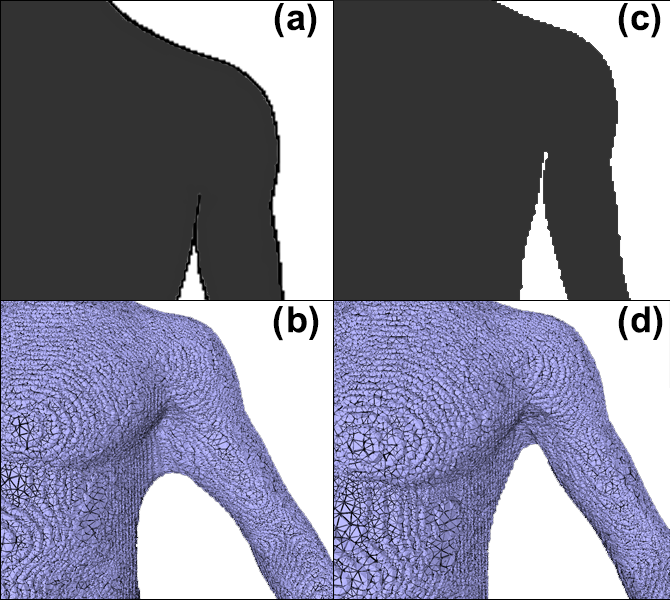
\includegraphics[width=0.85\textwidth]{IMG/volumetrizacion4.png}
    \caption{
    \emph{Voxelización} con el etiquetado de los \emph{vóxeles} de la piel (a) y la malla de tetraedros generada (b) conectando zonas próximas. \emph{Voxelización} sin etiquetar los \emph{vóxeles} de la piel (c) y la malla de tetraedros (d) resultante.
    \label{fig:volsol}
    %\emph{Volumetrización} de la zona de la axila. En la columna de la izquierda muestra el problema de no eliminar los \emph{vóxeles} etiquetados como piel. En la columna de la derecha, la zona de la axila no se encuentra interconectada
    }

\end{figure}
%(ver fig. \ref{fig:volsol}).}
%
%En la etapa de \emph{volumetrización} (sec. \ref{posing:volumetrizacion}) se ha modificado la \emph{voxelización} para borrar los \emph{vóxeles} etiquetados por el borde de la piel. Por tanto, 
%En la figura \ref{fig:voxelizacion}.c se puede observar que los \emph{vóxeles} marcados como piel son etiquetados de nuevo como vacío con el objetivo de no crear tetraedros entre zonas próximas pero no conectadas. 




En la figura \ref{fig:volsol} se puede observar la diferencia en la malla volumétrica con y sin la solución planteada. En la imagen \ref{fig:volsol}a, se muestra la  \emph{voxelización} de la axila con \emph{vóxeles} de la piel etiquetados, lo que se traduce en una generación de tetraedros que conectan el brazo con el pecho, como se puede ver en la imagen \ref{fig:volsol}b. En la imagen \ref{fig:volsol}c  se puede observar la \emph{voxelización} dejando la piel sin etiquetar y, por tanto, en la figura \ref{fig:volsol}d la zona de la axila está correctamente separada.
%

%





%

%Debido a la necesidad de que el algoritmo resulte robusto frente a los problemas citados, se ha procedido a añadir diferentes ajustes en el algoritmo propuesto en varias de sus etapas.

Con esta modificación se resuelven problemas de interconexión entre zonas no conectadas, aunque podría generar situaciones donde se puedan encontrar tejidos que no están dentro de la malla volumétrica. %Esta solución genera un problema  adicional al crear situaciones donde se puedan encontrar ciertos tejidos fuera de la piel. 

%Con esta modificación, 
En el caso concreto del modelo \emph{ZygoteBody}$^{TM}$ Masculino, alrededor de un 4.6\% de los vértices del modelo se sitúan fuera de la malla volumétrica. 
Este incremento no afecta de manera significativa el proceso de \emph{mapeado} y se detallará en la sección  \ref{sec:rendimiento}.

Otra limitación de los modelos de entrada, es que generalmente no se dispone de imágenes médicas del paciente completo debido a que muchos de los procedimientos médicos se realizan solo en áreas localizadas.
%muchas de las imágenes médicas disponibles no representan completamente el modelo anatómico del paciente. ç
El algoritmo propuesto es capaz de tratar con información incompleta, como se puede observar en la figura \ref{fig:patient} donde se muestra un modelo construido a partir de imágenes médicas reales. Este modelo fue creado con la suite \ac{ITGVPH} del proyecto \ac{RASimAs}.

%%%%%%%%%%%%%%%%%%%%%%%%%%%%%%%%%%%%%
\begin{figure}[ht]
   \centering
    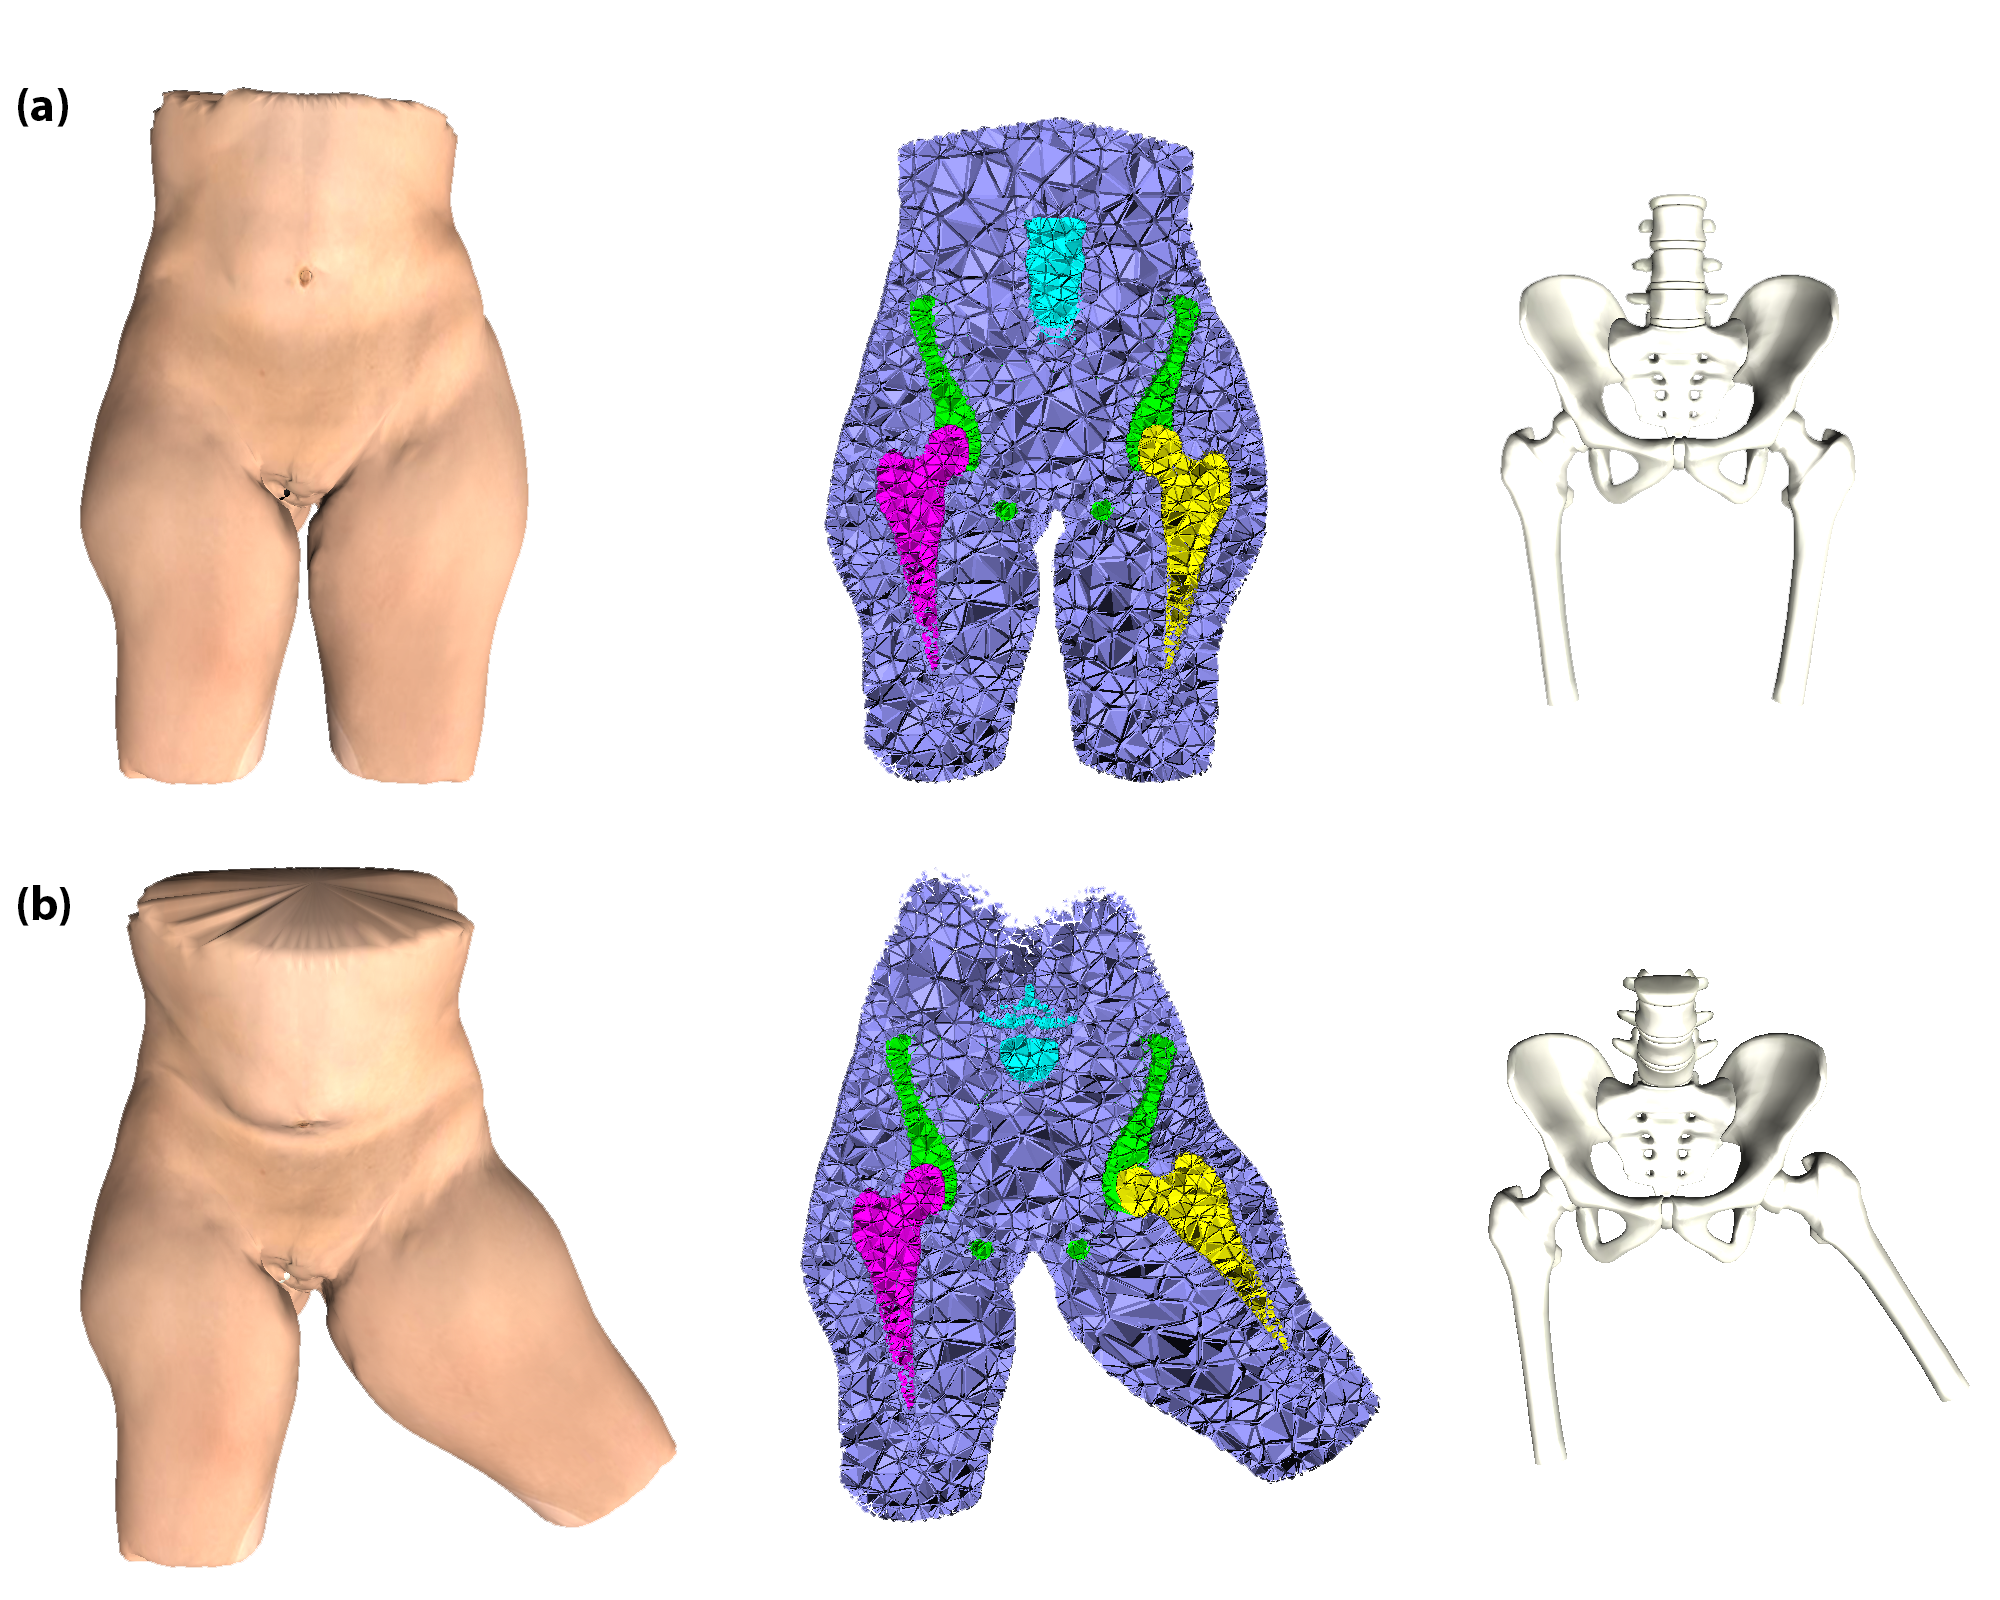
\includegraphics[width=0.9\textwidth]{IMG/patient.png}
    \caption{En la fila superior (a) se muestra el paciente virtual construido a partir de datos de un paciente real en posición de reposo y la \emph{volumetrización} generada. En la zona inferior, se puede observar como la pierna ha sido re-posicionada utilizando el algoritmo propuesto en este trabajo.
    }
   \label{fig:patient}
\end{figure}


%Estos vértices no afectan de manera determinante en el proceso de mapeado. 


%%%%%%%%%%%%%%%%%%%%%%%
%Comparación entre técnicas
%%%%%%%%%%%%%%%%%



A continuación, se van a analizar los resultados que produce el algoritmo utilizando los diferentes métodos de \emph{skinning} (\ac{COR}, \ac{LBS} y \ac{DQS}).
%
%La etapa de selección de poses del algoritmo incluye la fase de \emph{skinning} para los vértices de los tetraedros y la consecuente deformación que es transferida a los tejidos del modelo virtual. 
Primero, para mostrar de manera simple las diferencias visuales que se generan a través de las tres técnicas anteriormente citadas, se va a utilizar un prisma rectangular con cuatro huesos virtuales en su interior. Este modelo  se utilizará por su simplicidad para mostrar los resultados de rotaciones y giros con la finalidad de visualizar de forma directa las diferencias entre las técnicas seleccionadas. En la figura \ref{fig:bar_bending} se pueden observar las diferencias visuales del método seleccionado \ac{COR} frente a los métodos \ac{LBS} y \ac{DQS}. En cuanto a las rotaciones, se puede apreciar que en el caso de \ac{LBS} la articulación se colapsa (llamado normalmente \emph{collapsing elbows}). Sin embargo, en \ac{DQS} las articulaciones no se colapsan, pero se puede observar un abultamiento (este efecto se conoce como \emph{joint-bulging effect}). Respecto a los giros, es conocido que la técnica \ac{DQS} solvente el problema de \ac{LBS} donde la interpolación lineal de las matrices de transformación produce el efecto \emph{candy-wrapper}. Se puede observar que la técnica \ac{COR} solventa de forma adecuada los tres efectos (\emph{collapsing elbows}, \emph{joint-bulging effect} y \emph{candy-wrapper}). 
En esta figura (fig. \ref{fig:bar_bending}), se muestra el resultado sobre la malla de tetraedros. Estos se colorean según el peso de sus vértices, mostrando las diferentes influencias de los huesos virtuales. Se ha usado un código de colores: el color azul muestra donde los huesos impares alcanzan mayor influencia y el color rojo es donde los huesos pares alcanzan su mayor influencia. %Con este código de colores se puede observar las transiciones entre huesos de color verde.
Las transiciones entre áreas de influencia de dos huesos se pintan en verde.

\begin{figure*}[ht]%[b]%[b!ht]
  \centering
  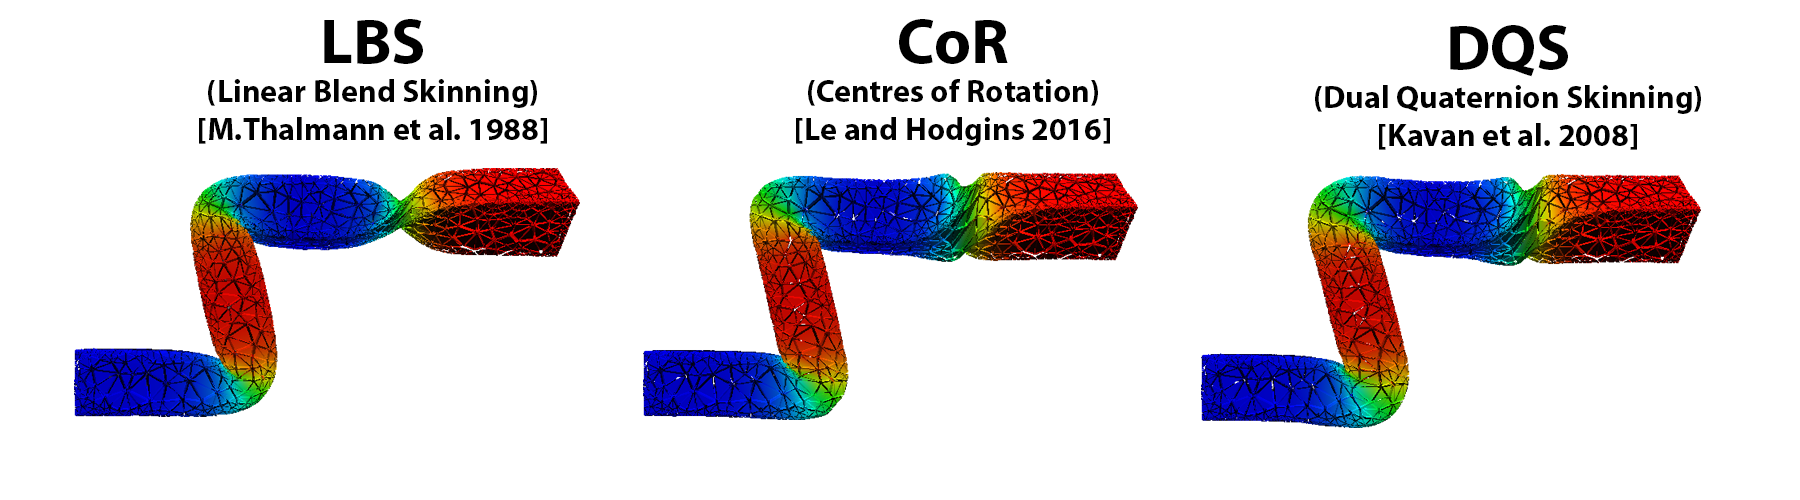
\includegraphics[width=\textwidth]{IMG/BarraCoR}
    \caption{Deformación del modelo de barra por las 3 técnicas. Primera rotación de 100º, segunda rotación de -100º y un giro de 135º. En rojo, los tetraedros influenciados por los huesos pares, y en azul aquellos influenciados por los huesos impares. Las transiciones se muestran en verde.}
    \label{fig:bar_bending}
\end{figure*}
%%%%%%%%%%%%%%%%%%%%%%%%%%%%%%%%%%%%%

El objetivo de la utilización de esta forma geométrica sencilla es mostrar de forma clara las diferencias que se obtienen de las distintas técnicas de \emph{skinning}. %A continuación, se mostrarán los resultados obtenidos al utilizar estas mismas técnicas utilizando los modelos anatómicos. 
En las siguientes figuras, se utilizarán diferentes posturas de los modelos anatómicos para mostrar las diferencias en los resultados que producen cada uno de los métodos al deformar el paciente virtual.

En la figura \ref{fig:thigh_bending} se muestra una rotación de la articulación de la pierna. Las zonas susceptibles de mostrar defectos son la zona superior del muslo en la zona inguinal y el glúteo. En esta imagen se puede observar que tanto en la zona inguinal como en el glúteo con la técnica \ac{LBS} se produce el efecto \emph{collapsing elbows}. En el caso de utilizar \ac{DQS}, se aprecia el defecto \emph{joint-bulging effect} común de esta técnica. Sin embargo, la técnica \ac{COR} ofrece un compromiso entre ambas. La imagen se acompaña con el tejido muscular en reposo como referencia y la deformación de los tejidos circulatorio y nervioso, como ejemplo de tejidos internos del modelo. En esta última imagen, no se han incluido sus diferentes deformaciones ya que las diferencias visuales entre técnicas de estos dos tejidos es mínima al ser estructuras filiformes. En la figura \ref{fig:axila} se muestra otra deformación del modelo \emph{ZygoteBody}$^{TM}$ Masculino. En este caso, en la axila, la técnica \ac{DQS} genera un abultamiento donde las técnicas \ac{LBS} y \ac{COR} no producen efectos no deseados.



% %%%%%%%%%%%%%%%%%%%%%%%%%%%%%%%%%%%%%
\begin{figure*}[ht]%[b]%[b!ht]
  \centering
  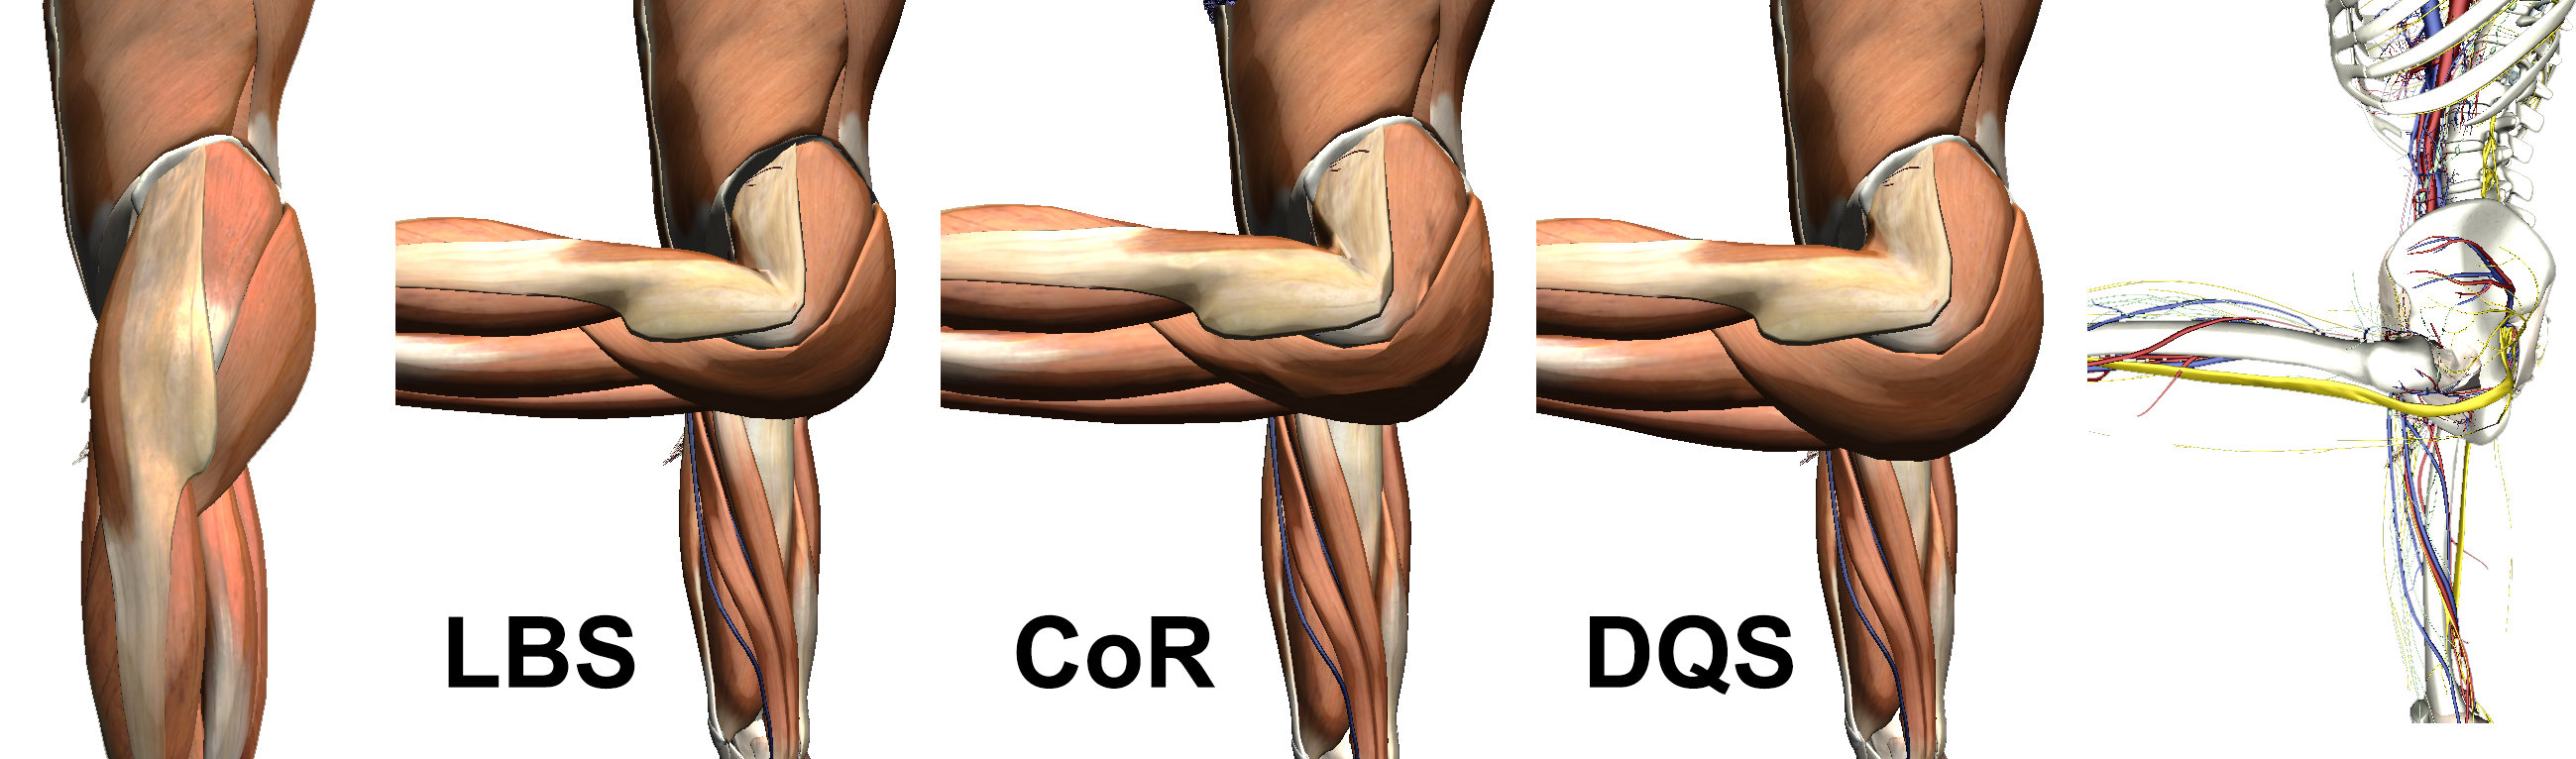
\includegraphics[width=\textwidth]{IMG/compculo}
    \caption{ Rotación de la pierna izquierda. En la primera imagen se encuentra la posición de reposo. A continuación, de izquierda a derecha se muestran la pierna rotada usando las 3 técnicas de \emph{skinning} (en \acs{LBS}, la articulación colapsa tanto en el glúteo como en la zona inguinal, \acs{DQS} produce un abultamiento en el glúteo y \acs{COR} suaviza esos defectos). A la derecha, se ocultan los músculos para mostrar el tejido nervioso y circulatorio con la misma deformación producida por \acs{COR}.}
    \label{fig:thigh_bending}
\end{figure*}

\begin{figure*}[ht]%[b]%[b!ht]
  \centering
  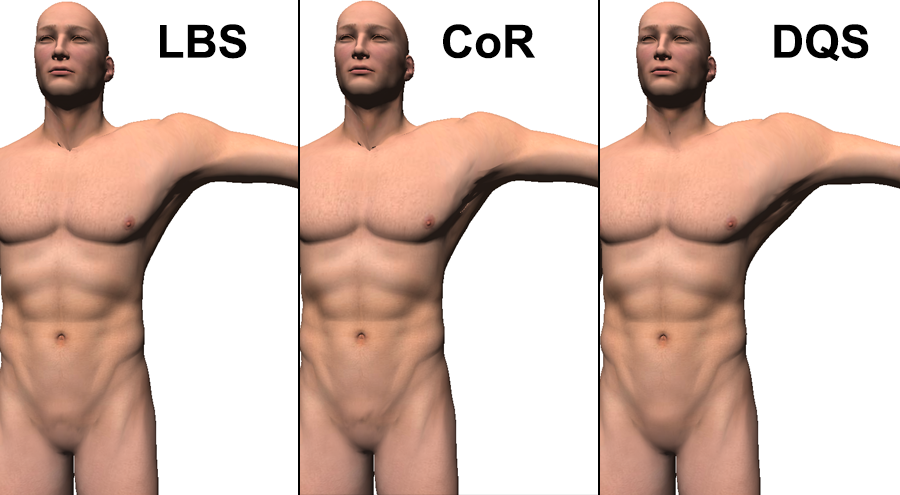
\includegraphics[width=0.8\textwidth]{IMG/sobaco.png}
    \caption{Ejemplo de deformación del  \emph{ZygoteBody}$^{TM}$ Masculino. En la zona de la axila, \acs{DQS} sufre un abultamiento (\emph{joint-bulging effect}) que no producen las técnicas \acs{COR} y \acs{LBS}. }
    \label{fig:axila}
\end{figure*}
%%%%%%%%%%%%%%%%%%%%%%%%%%%%%%%%%%%%%




%\del{Con los resultados obtenidos, se puede afirmar que el algoritmo propuesto obtiene deformaciones visualmente realistas y es capaz de realizarlas en tiempo de ejecución delegando las etapas más pesadas a un proceso previo.}


%%%%%%%%%%%%%%%%%%%%%%%%%%%%%%%%%%%%%
\begin{figure}[!ht]%[ht]%[b]
   \centering
   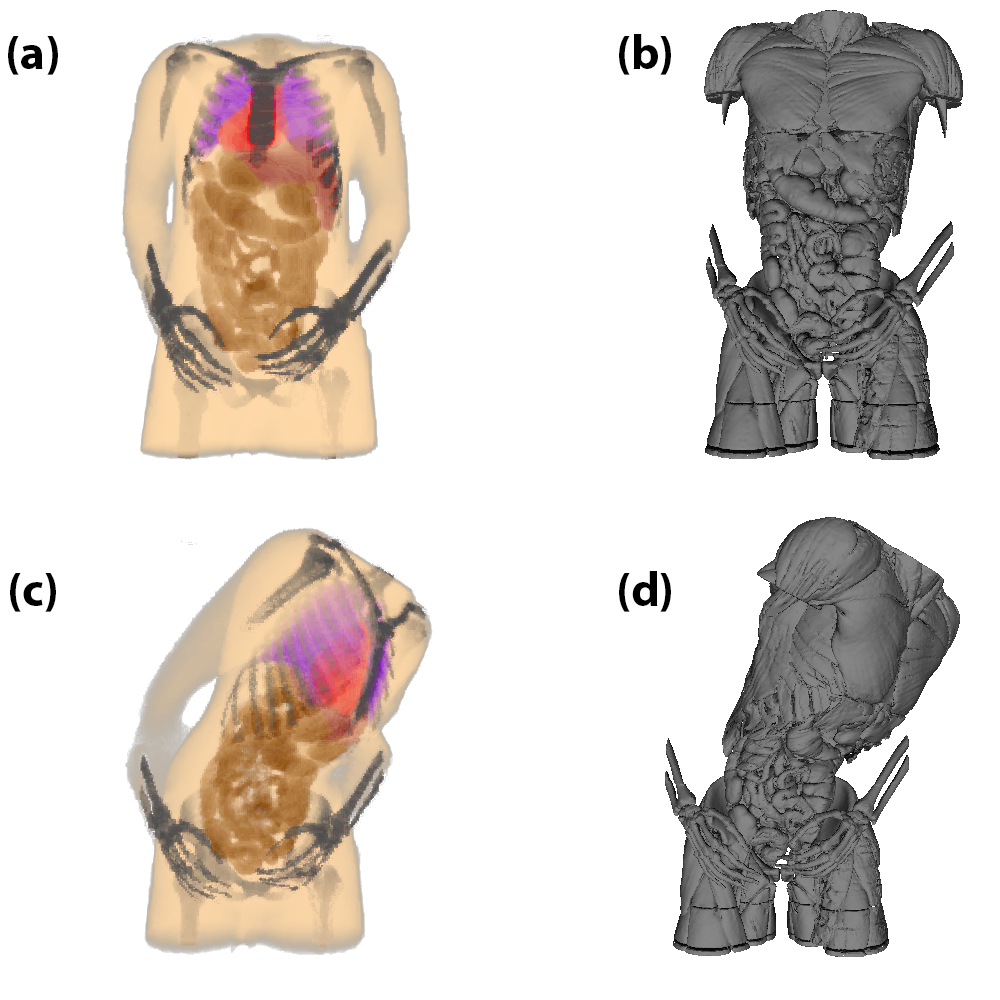
\includegraphics[width=0.8\textwidth]{IMG/HV}
    \caption{Algoritmo aplicado a diferentes representaciones: volumétrica (a) y (c), superficial (b) y (d). Imágenes (a) y (b) muestran el \emph{Segmented Inner Organs} en posición de reposo. Imágenes (c) y (d) muestran el resultado del modelo deformado.}
    \label{fig:humanvisible}
\end{figure}

Con la intención de seguir mostrando las capacidades del algoritmo propuesto, se presentan más ejemplos de deformaciones realizadas para esta tesis. En la figura \ref{fig:humanvisible}, se puede observar tanto el modelo superficial como el volumétrico de los datos del modelo \emph{Segmented Inner Organs}(\cite{VM2002},~\cite{VoxelMan}). Este caso demuestra la flexibilidad del algoritmo propuesto al tratar con datos incompletos, y la posibilidad de poder tratar tanto con mallas superficiales como con representaciones volumétricas.
%
Finalmente, en la imagen \ref{fig:run1} se muestran resultados adicionales del uso del algoritmo con la técnica de \emph{skinning} \ac{COR} en los modelos \emph{ZygoteBody}$^{TM}$ Masculino y Femenino en diferentes situaciones.

%%%%%%%%%%%%%%%%%%%%%%%%%%%%%%%%%%%%%
\begin{sidewaysfigure}[ht]%[b]%[b!ht]
   \centering
   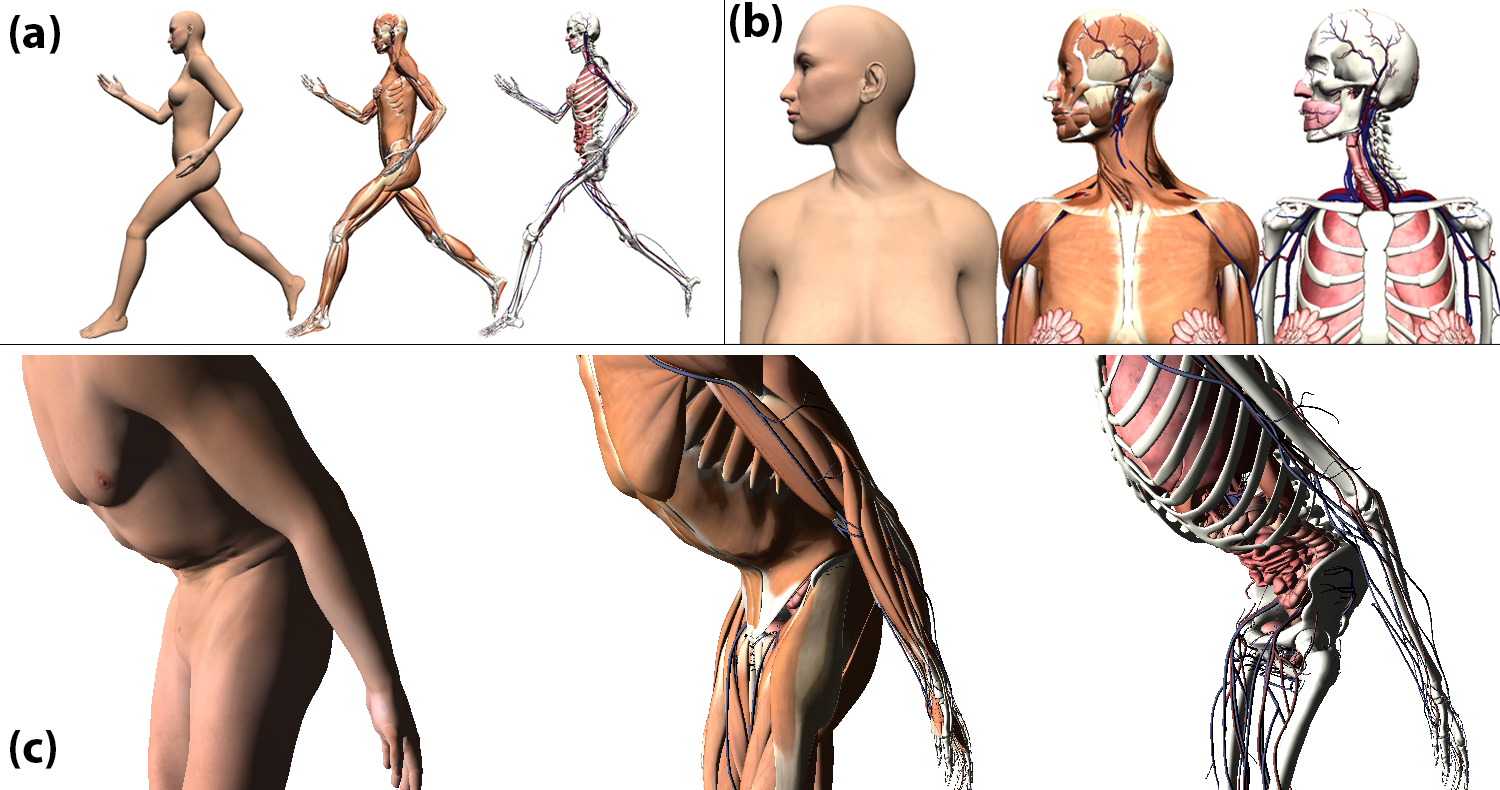
\includegraphics[width=0.90\textwidth]{IMG/examples}
    \caption{Resultados obtenidos utilizando \acs{COR}. (a): fotograma del ciclo de carrera (\emph{ZygoteBody}$^{TM}$ Femenino). (b): Ejemplo de rotación de cuello (\emph{ZygoteBody}$^{TM}$ Femenino). (c): Zona abdominal flexionada (\emph{ZygoteBody}$^{TM}$ Masculino).}
    \label{fig:run1}
\end{sidewaysfigure}
%%%%%%%%%%%%%%%%%%%%%%%%%%%%%%%%%%%%%
\clearpage


%%%%%%%%%%%
%%%%%%%%%%%%
%%%%%%%%%
Las deformaciones resultantes de la etapa anterior dan como resultado poses visualmente plausibles en la mayoría de los casos. 
%Aun así, se ha incluido la fase de optimización que permita al usuario deformar el paciente virtual con una técnica basada en físicas aunque no se dispongan de las descripciones mecánicas. A continuación, se mostraran la comparación de los resultados obtenidos y una evaluación para conocer si el usuario prefiere esta fase adicional frente a la solución geométrica.
La fase de \emph{skinning} basada en \ac{COR} solventa de forma efectiva los problemas típicos de las técnicas basadas en \ac{LBS} y de \ac{DQS}. Aún así, en algunas circunstancias se han detectado comportamientos no deseados que se aprecian visualmente como un aumento o disminución de volumen. 
La técnica \ac{COR} no puede asegurar la conservación de volumen tal y como lo hacen las técnicas basadas en física. %debido a que no se tiene en cuenta. 
En el algoritmo propuesto, se ofrece la posibilidad de ejecutar una etapa adicional no interactiva para refinar los resultados obtenidos.
Debido a que no se puede asegurar una apropiada descripción mecánica de los tejidos, el objetivo de esta optimización es garantizar la conservación del volumen utilizando la formulación co-rotacional del \acs{FEM} (ver sec. \ref{posing:optimizacion}).

La figura \ref{fig:anatomium} ilustra un ejemplo de cómo la técnica basada en la formulación \ac{FEM} muestra diferencias con el resultado obtenido con la técnica \ac{COR}. Aun así, en la mayoría de los casos, ambas técnicas producen resultados similares. En la siguiente sección, se mostrarán los resultados que se han obtenido al realizar un estudio para conocer si el usuario prefiere esta fase adicional frente a la solución geométrica.


%Se ha propuesto utilizar la formulación \ac{FEM} co-rotacional para resolver el problema estático considerando un material lineal, isotrópico y homogéneo. %Se ha escogido el módulo de \emph{Young}  intentado mejorar la estabilidad del sistema. Para ello, se han analizado distintas matrices de coeficientes del sistema, obtenidas a partir de distintos valores del módulo de \emph{Young}, quedándose con el valor que daba como resultado la matriz de coeficientes con menor número condicionante. 
%En la mayoría de los casos probados, solo se necesitaba una iteración al resolver el sistema. Los resultados obtenidos con más iteraciones eran prácticamente indistinguibles. 
 
%  Besides, the deformations are measured using the \emph{Cauchy} strain tensor. The boundary conditions, needed to solve the steady-state problem, are given by the positions of the vertices labelled as bones. The co-rotational formulation calculates the internal forces caused by the deformations in a non-rotated configuration. Then, the internal forces are rotated again into the final configuration \cite{Muller2004}. The algorithm needs to compute the element rotations in the final configuration. For this purpose, the solution is refined iteratively. The elastic used model can be tuned with two parameters: the \emph{Poisson ratio}  and the \emph {Young module}. The \emph{Poisson ratio} controls the volume conservation and it should take a value close to 0.5 (the real value has to be lower to ensure numeric stability). Since the material is homogenous, this value has no impact on the outcome. 

 %Sin embargo, debido a que ambos resultados son plausibles se ha procedido a enunciar la siguiente hipótesis: los resultados de la etapa de optimización serán elegidos por los usuarios frente a la técnica geométrica.
 
\begin{figure}[ht]%[b]%[b!ht]
   \centering
   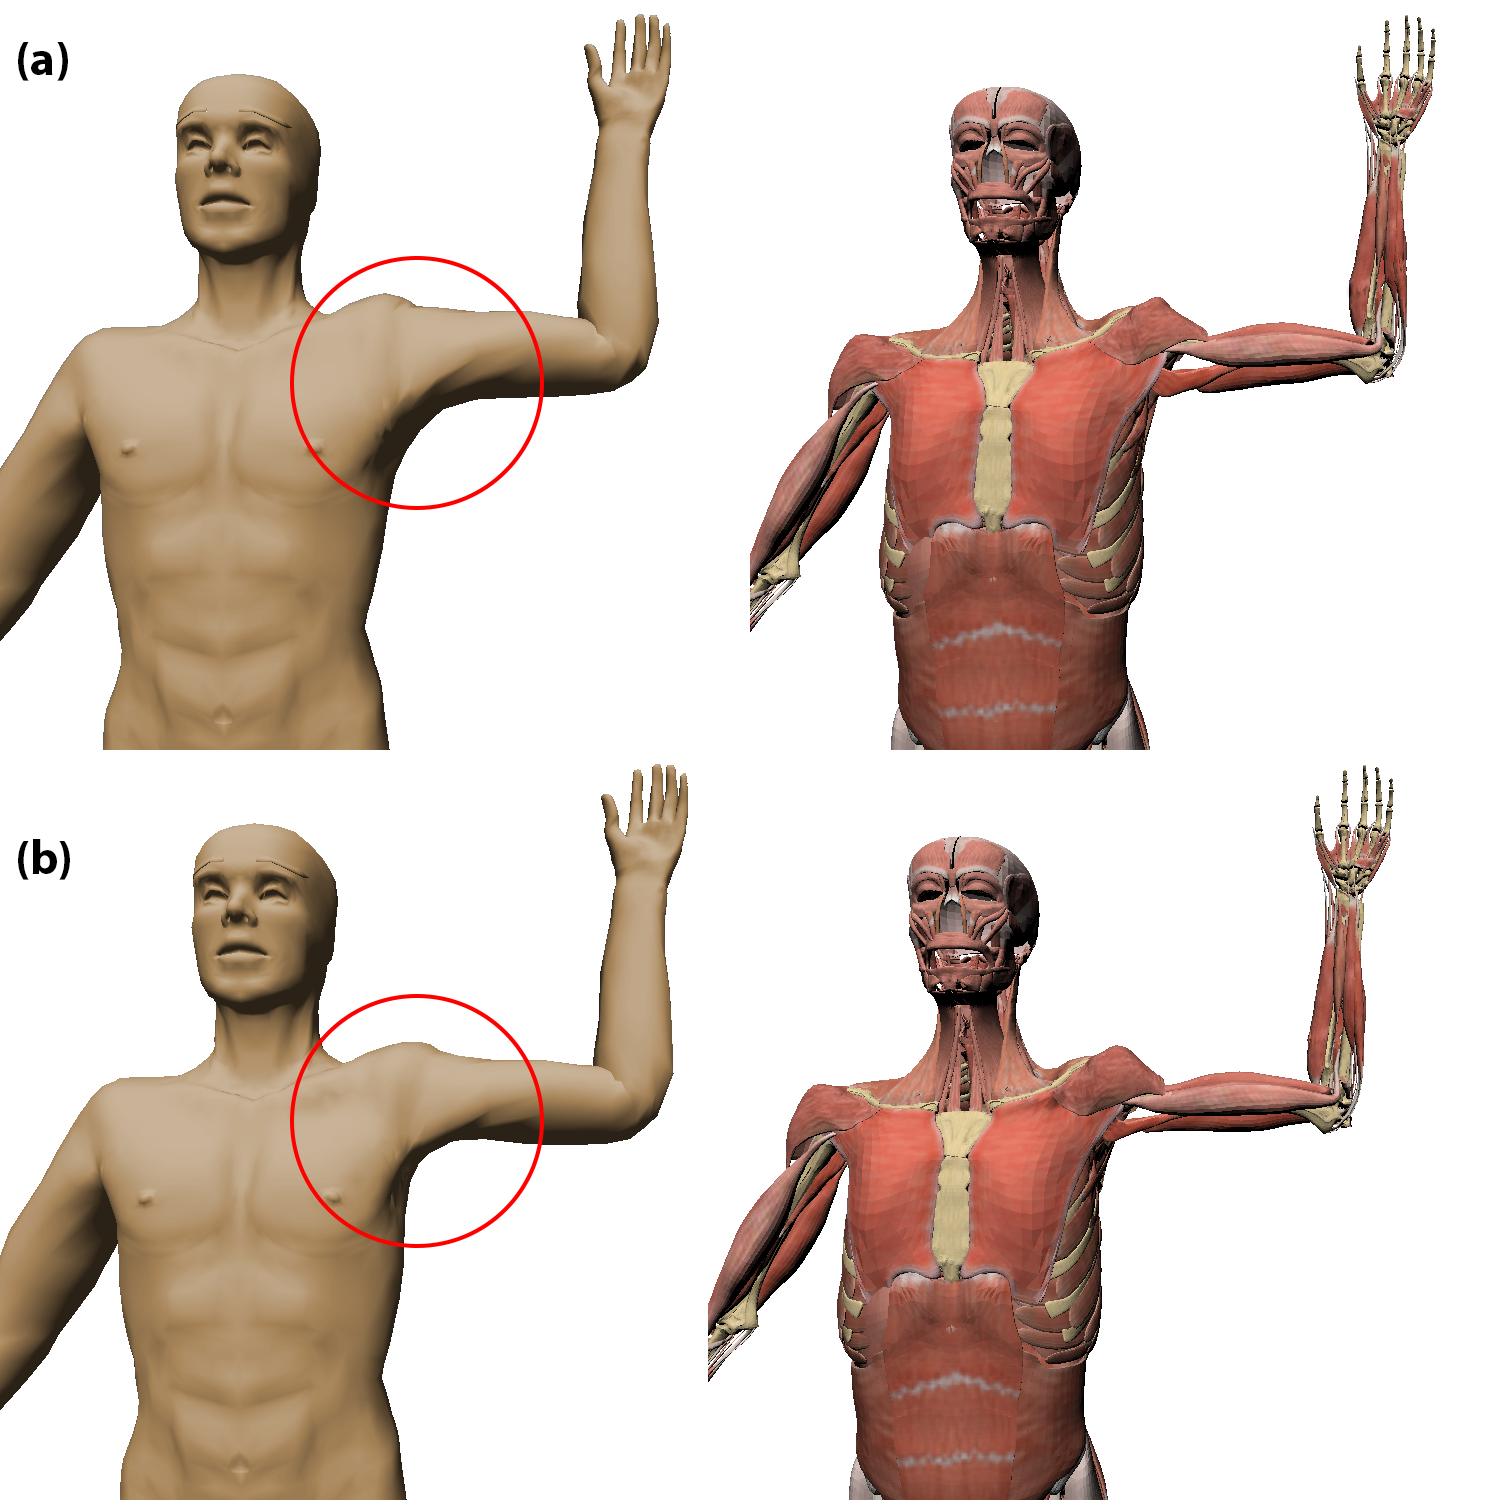
\includegraphics[width=0.9\textwidth]{IMG/AntCOR}
    \caption{ Comparación entre \acs{COR} (a) y la técnica \acs{FEM} (b) diseñada para conservar el volumen. \acs{COR} incrementa ligeramente el volumen en la zona de la axila.}
    \label{fig:anatomium}
\end{figure}

\subsection{Evaluación perceptual}


%
Como se ha introducido anteriormente, la técnica \ac{COR} muestra, en ocasiones, cambios de volumen, que se intentan solventar con una etapa de optimización sacrificando conseguir tasas de refresco interactivas. Estos casos no son muy comunes y en la mayoría de ocasiones ambas soluciones proporcionan resultados indistinguibles, con la diferencia de que la etapa de optimización requiere unos cálculos costosos. 
%\todo{importante para simuladores de importancia}
Para comprobar si los usuarios son capaces de distinguir entre técnicas, se ha procedido a realizar un estudio entre distintos usuarios. La encuesta se puede consultar en el apéndice \ref{anexo:cuestionario}.

En esta encuesta, se ha pedido a los participantes que valoren el realismo de varias imágenes estáticas basándose en una escala de tipo \emph{Likert} comprendida entre los valores 1 y 8. Primero, se mostraba una imagen con el paciente virtual en reposo
%la imagen de referencia para cada deformación 
y, a continuación, se presentaban dos  imágenes. Estas imágenes correspondían a una deformación obtenida por ambas técnicas: la optimización \ac{FEM} y el resultado de la técnica \ac{COR}. Se mostraban posiciones diferentes, utilizando los modelos junto con sus tejidos internos: \emph{ZygoteBody}$^{TM}$ Masculino y Femenino; Anatomium; y el modelo extraído de paciente real. Para reducir el sesgo de orden, las imágenes se mezclaban de manera aleatoria.


Un total de dieciséis sujetos han participado, de los cuales dos eran mujeres y catorce eran hombres;
%\todo{Metemos la gráfica de la otra encuesta? quito la primera encuesta de los anexos?}. 
con una edad comprendida entre los 20 y los 52; donde trece de ellos se han identificado como profesionales de informática gráfica.


En primer lugar, se ha comprobado si las respuestas representaban una distribución normal. Al resultar negativo, se han comparado los resultados obtenidos utilizando la prueba de los rangos con signo de Wilcoxon no paramétrica para comparar el rango medio de dos muestras relacionadas y determinar si existen diferencias entre ellas. Con el resultado obtenido (\emph{p-value} $> 0.9$ intervalo de confianza) no se puede confirmar que los usuarios encuentren diferencias significativas entre ambos modelos. 
En la figura \ref{fig:stat} se muestran los resultados de la encuesta en una representación con dos diagramas de cajas y bigotes. En el diagrama (a), se han agrupado las respuestas de cada una de las técnicas. Por otra parte, en el diagrama (b), se muestran las respuestas separadas por poses de las distintas técnicas utilizadas. Como se puede observar, las valoraciones de ambas técnicas son similares, con lo que se puede concluir que los usuarios no encuentran diferencias significativas entre ambas.  
%

%

\begin{figure}[ht]%[b]%[b!ht]
   \centering
   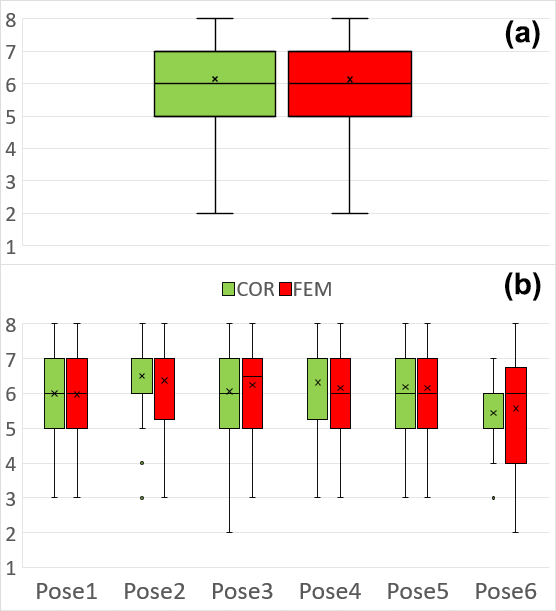
\includegraphics[width=0.9\textwidth]{IMG/boxplot}
    \caption{Diagramas de cajas y bigotes comparando los resultados de la encuesta. El diagrama (a) muestra todas las respuestas agrupadas por técnica. El diagrama (b) compara el resultado de ambas técnicas por cada pose diferente.}
\label{fig:stat}
   \end{figure}
%\subsection{Proceso previo}

\clearpage


\subsection{Rendimiento}
\label{sec:rendimiento}

Uno de los principales objetivos del algoritmo propuesto es que la selección de poses pueda ejecutarse interactivamente. Así pues, en el cauce de animación propuesto se han delegado las etapas más costosas computacionalmente a un proceso previo. Este preproceso generará un conjunto de datos auxiliares que serán usados por la herramienta al seleccionar el modelo virtual asociado. Solo se necesita ejecutar el preproceso una vez por modelo anatómico, %Estos datos solo son necesarios crearlos una vez por modelo,
pudiendo cargar el paciente virtual tantas veces como se necesite sin volver a generar estos datos. Aun así, algunas fases de la etapa de preproceso han sido diseñadas para minimizar el tiempo de ejecución.


Como se ha citado en la sección \ref{sec:ana_prev}, la modificación para quitar los \emph{vóxeles} de la piel en la \emph{voxelización} (ver sec. \ref{posing:volumetrizacion}) produce vértices huérfanos que se encuentran fuera de la malla de tetraedros.
Debido a este problema, se propuso una modificación adicional de la etapa de mapeado (ver sección \ref{posing:Mapeado}). Aprovechando la estructura espacial que proporciona la \ac{tabla hash}, aunque el vértice no esté dentro de ningún tetraedro, es fácil buscar el tetraedro más cercano recursivamente en la \ac{tabla hash}. 
En este caso, el tiempo de mapeado es 36,35 segundos utilizando la \ac{tabla hash} como método de búsqueda. Este tiempo es muy pequeño si se compara con el tiempo que tardaría  la técnica de fuerza bruta, que sería de 4 horas y 55 minutos para relacionar 1 277 325 de vértices a 2 584 115 de tetraedros. % en el caso del mismo ejemplo. 

\begin{table*}[ht]
\begin{threeparttable}
\centering
\caption{Comparación de tiempos de mapeado entre la técnica de \emph{Spatial Hashing} y el algoritmo de fuerza bruta. }
\label{tab:bruteforce}
\begin{tabular}{|c|c|x{25mm}|x{25mm}|x{25mm}|}
\hline
\textbf{Modelo} & \textbf{Vértices} & \textbf{Vértices  huérfanos (\%)}  & \textbf{Spatial Hashing (ms)} & \textbf{Fuerza bruta (ms)} \\ 
\hline
Piel             &32 748      &89.81   &10 678* &547 967\\
\hline
Músculos         &311 600     &2.02    &12 157* &4 088 365\\ 
\hline
S. nervioso      &379 008     &1.41    &12 814* &5 140 770\\ 
\hline
Tejido conectivo &168 343     &0.68    &7 881*  &2 210 942\\ 
\hline
S. linfático     &5 324       &5.66    &5 456*  &702 087\\ 
\hline
S. circulatorio  &380 302     &4.29    &11 541* &5 008 874\\ 
\hline
\textbf{TOTAL}   &1 277 325    &4.6     &36 357  &$17.7*10^6$ \\
\hline
\end{tabular}
\begin{tablenotes}
      \small
      \item * La creación de la \ac{tabla hash} está incluida en cada medición (4 834 ms). El tiempo total no puede ser calculado directamente sumando todos los valores de la columna.
\end{tablenotes}
\end{threeparttable}
\end{table*}

En la tabla \ref{tab:bruteforce} se muestra una comparación entre los tiempos empleados por el algoritmo de fuerza bruta y el método \emph{Spatial Hashing} en mapear los distintos tejidos del \emph{ZygoteBody}$^{TM}$ Masculino con su malla volumétrica. Como se puede observar, un gran porcentaje de los vértices de la piel se encuentran fuera de la malla de tetraedros. Este resultado es lógico al eliminar los \emph{vóxeles} que pertenecían a la piel. Sin embargo, los demás vértices huérfanos corresponden a la problemática ya citada del modelo anatómico. Esto solo hace reafirmar la robustez del algoritmo propuesto ante fallos del modelo de entrada. La complejidad de la malla de tetraedros se puede consultar en la tabla \ref{tab:complex}. 



Para finalizar de analizar el preproceso del algoritmo, a continuación, se muestra la tabla \ref{tab:pre_pro} dónde se pueden consultar los tiempos empleados en cada etapa utilizando los tres modelos más complejos de los que se disponía. Se obtienen resultados similares, los cuales se sitúan en torno a los siete minutos.

%\todo{meter todos los valores significativos de configuración}

%Los valores de configuración para las distintas etapas son las siguientes:
%La volumetrización no se hará en una caja contenedora más grande de tamaño 250x700x120. En cuanto a la función de similaridad empleada en la técnica de \emph{skinning} \ac{COR}, el valor de $\sigma$ que se utiliza es $0.1$. El \emph{ratio de Poisson} se estableció en 4.999 y el \emph{módulo de Young} en 0.01.



\begin{table*}[ht]
\begin{threeparttable}
\centering
\caption{Tiempo (en milisegundos) utilizado por cada etapa. }
\label{tab:pre_pro}
\begin{tabular}{|x{30mm}|c|c|c|c|c|}
\hline
\textbf{Modelo} & \textbf{Rigging} & \textbf{Volumetrización} & \textbf{Pesado} & \textbf{Mapeado} & \textbf{COR }  \\ 
\hline
\emph{ZygoteBody}$^{TM}$ Masculino  & 32 698 & 69 044 & 11 762  & 51 160   & 138 005 \\ 
\hline
\emph{ZygoteBody}$^{TM}$ Femenino  & 33 251 & 63 401 & 9 171  & 71 635   & 208 886  \\ 
\hline
Anatomium   & 31 891 & 120 465 & 23 318 & 44 521  & 115 214\\ 
\hline
\end{tabular}
\begin{tablenotes}
      \small
      \item *\acs{COR} es la etapa de calcular los centros de rotación (sec. \ref{posing:Poses}).
\end{tablenotes}
\end{threeparttable}
\end{table*}


En cuanto a la etapa de selección de poses, esta debe ser interactiva al ser necesaria la intervención de un usuario para supervisar la deformación de los tejidos. Es importante remarcar que el algoritmo propuesto puede manejar una gran cantidad de vértices y tetraedros como se puede observar en los datos de la tabla \ref{tab:complex}. En la tabla \ref{tab:inter} se muestra el rendimiento de los métodos utilizados \ac{COR}, \ac{LBS} y \ac{DQS}. Como se puede observar, las diferencias de rendimiento entre las tres técnicas son despreciables. La tabla muestra los valores máximos y mínimos de imágenes por segundo que es capaz de generar el algoritmo utilizando un ciclo de caminado para animar al modelo virtual.
%
\begin{table}[ht]
\centering
\caption{Valores máximos y mínimos de imágenes por segundo durante el ciclo de caminado en la etapa de \emph{selección de poses}.}
\begin{tabular}{|c|c|c|c|}
%\multirow{2}{*}{\textbf{Model}} & \multicolumn{2}{c}{\textbf{Interactive stage}} & \multirow{2}{*}{\textbf{Optimization}} \\
\hline
\textbf{Modelo}&\textbf{LBS} &\textbf{DQS} &\textbf{COR} \\ 
\hline
\emph{ZygoteBody}$^{TM}$ Masculino  & 111-90 & 100-90 & 100-76\\ 
\hline
\emph{ZygoteBody}$^{TM}$ Femenino  & 76-60  & 66-52   & 60-50 \\ 
\hline
Anatomium   & 166-142 & 166-125 & 142-100\\ 
\hline
\end{tabular}
\label{tab:inter}
\end{table}



%\subsection{Selección de poses}
% \subsection{Aspecto visual} \todo{Hay otro tipo de nombre para esta sección?}


% \subsection{Optimización}
% \label{posing:optimizacion}


%%%%%%%%%%%%%%%%%%%%%%%%%%%%%%%%%%%%%


%






%%%%%%%%%%%%%%%%%%%%%%%%%%%%%%%%%%%%% 








%Due to their high content of water, organic tissues can be considered incompressible. For that reason, volume conservation is a desirable feature. In this vein, we have compared the behaviour of LBS, DQS, CoR and our Optimization step (FEM). To this end, we used the same MoCap walk cycle to animate the previously mentioned models. The results of this test are shown in Fig.  \ref{fig:volRatio}.
%\textcolor{red}{It can be observed how the optimization stage solve the volume problems of LBS and DQS. VER QUE PASA CON COR. }
%\begin{figure*}%[!ht]
%   \centering
%    \includegraphics[width=0.98\textwidth]%{img/graficas}
%    \caption{Volumen conservation rate of %the several \emph{skinning} techniques. }
%     \label{fig:volRatio}
%\end{figure*}

% \subsection{Discusión}
% \label{posing:discusion}
% \todo{Hablar de la necesidad de validación}


% A partir de los resultados que se han mostrado en la sección anterior, se puede afirmar que el algoritmo puede generar una cantidad infinita de variaciones de un mismo modelo anatómico, siendo posible aunque el modelo sea incompleto o no se disponga de sus propiedades mecánicas. Además, el cauce diseñado hace que la etapa de selección de poses permita a cualquier usuario animar pacientes virtuales de forma interactiva.


% La técnica de posicionamiento de pacientes virtuales se diseñó con el objetivo de ser lo más flexible posible, minimizando los requisitos de los datos de entrada. La clave de está flexibilidad radica en que se calcula un campo de deformaciones continuo dentro del modelo anatómico. Este campo permite adaptar cualquier tejido a la pose deseada, de forma independiente al resto de tejidos, pudiendo así trabajar con modelos incompletos. En este sentido, la única limitación que se impone es que tanto la piel como el tejido óseo del paciente virtual deben de estar segmentados. Esta restricción no debería suponer un gran problema, dado que estos tejidos son visibles en la mayor parte de las técnicas de imagen médica.

% La utilización del campo de deformaciones aporta beneficios adicionales. Evitar colisiones y autocolisiones en los tejido transformados es de vital importancia de cara a garantizar el buen funcionamiento del simulador físico y del simulador de \ac{US} de \ac{RASimAs}. De esta forma, solo podrán aparecer colisiones y/o autocolisiones si: (i) se utilizan mallas para representar los tejidos con una resolución inadecuada o (ii) si existen colisiones y/o autocolisiones en el modelo virtual de partida. Debido a que la extracción de los tejidos desde imágenes médicas no es perfecta, pueden aparecer las auto colisiones y colisiones entre tejidos. La técnica propuesta no solventa estas colisiones, pero es robusta en su tratamiento. Aun así, las colisiones con el tejido óseo y muy especialmente con la piel, pueden provocar una importante perdida de realismo. Cabe destacar, que, a pesar de esta circunstancia, la técnica propuesta es mucho más robusta, en este escenario, que los métodos basados en simulación física. %En la sección \ref{posing:method}, se proponen técnicas para mitigar estos problemas.

% Tal y como se muestra en la sección \ref{posing:animvol}, este campo puede aplicarse tanto a \ac{B-rep}s como a datos volumétricos. De esta manera, se ha extendiendo el alcance de la técnica propuesta.




%\todo{Esto se va al final de capítulo en la discusión. Lo vamos a meter con las limitaciones de la técnica. }
% \new{Por último, se han identificado las siguientes limitaciones:}
% \begin{itemize}
%     \item Las estructuras mínimas que necesita el algoritmo son la piel y los huesos. Estos tejidos son los más habituales que se pueden capturar en muchas de las imágenes médicas, por tanto, servirán para guiar el proceso e identificar algunos puntos claves para el correcto funcionamiento del algoritmo.
    
%     \item Debido a que la extracción de los tejidos desde imágenes médicas no es perfecta, se permiten que haya auto colisiones y colisiones entre tejidos. Aun así, se espera que los diferentes tejidos anatómicos no sobresalgan de la piel, ya que el algoritmo no está diseñado para resolver colisiones, además de no generar colisiones adicionales. Aunque aquellos tejidos que traspasen la piel son irreales, se tratarán por igual aunque no se puede asegurar una deformación realista.
    
%     \item El algoritmo utilizará un esqueleto virtual para definir los movimientos de las articulaciones. Se utilizará la información que proporciona los tejidos óseos para construir un esqueleto virtual adecuado al modelo de entrada. La principal limitación es la selección manual de las zonas identificadas que se necesitan para identificar los puntos de rotación de la articulación y su sistema de referencia.
% \end{itemize}



% Hay que remarcar que es necesario una validación formal para comprobar que esta técnica puede ser utilizada en simuladores médicos. De esta forma, se podrá comprobar que estas deformaciones puedan ser utilizadas en simuladores en el contexto de entrenamiento de un procedimiento médico. En las siguientes secciones, se utilizarán dos casos de uso propuestos con este objetivo

%\todo{La palabra realista me suena poco cientifica. Plausibles es un resultado que un usuario pueda interpretar como real.  }
%\del{A la vista de los resultados, se puede afirmar que el algoritmo propuesto cumple con la función de generar resultados visualmente \del{realistas}\new{plausible} que en el contexto de entrenamiento puede ser utilizadas para que la transferencia de habilidades de los simuladores que la utilicen sea efectiva. } %\todo{Como puedes afirmar que estos resultados son validos para el entrenamiento!!!!!!!! Has entrenado a médicos y después lo has evaluado!!!!! Aaron cuidado con lo que pones. La hipótesis es esa porque el objetivo era probar este sistema en herramientas reales. Hasta que no haya resultados en un simulador la hipótesis no queda probada!!!!!}

% En cuanto a la variabilidad anatómica, este  algoritmo ha sido incorporado en la herramienta \ac{TPTVPH} que va a ser integrada en el \ac{ITGVPH} que tiene como objetivo crear una base de datos de pacientes virtuales que posteriormente podrá ser utilizada en el simulador \ac{RASim}. Esta herramienta podría ser incorporada en otros simuladores que puedan beneficiarse de la adaptación de modelos anatómicos.
% Según los requisitos del proyecto \ac{RASimAs}, la herramienta \ac{TPTVPH} debe permitir a un usuario elegir la postura del paciente virtual de manera interactiva.% Además, se permitirá configurar el paciente virtual con posturas preselecionadas, para que sea posible su ejecución de manera completamente automática. Al igual que se muestra en la sección \ref{posing:result}, se pueden cargar poses provenientes de \ac{MoCap} o se pueden guardar posturas manualmente creadas.}
% En el capítulo siguiente, se describirá como se ha incluido la solución presentada en el desarrollo de la herramienta \ac{TPTVPH}.

% Por otra parte, con el objetivo de formar parte de herramientas interactivas, este método se puede incorporar en cualquier simulador que requiera cambiar la pose de un determinado modelo anatómico con estructuras internas en tiempo real. Para demostrar esta funcionalidad, se presentará un simulador de radiología diagnóstica que utiliza las ventajas del algoritmo propuesto.

%%%%